Many architectures and operating systems expose virtual memory and paging
abstractions. While most interfaces are fairly similar, we will use the
RISC-V ISA (privileged architecture version 1.10\cite{riscv_priv110}), and
Linux version 4.15\cite{linux} for most examples in this paper.

Figure \ref{fig:generic_paging_flow} shows a typical flow for translating a
virtual address. Most translations occur completely in hardware and require no
immediate OS intervention. However, when physical memory is constrained, the
operating system may choose to store logical pages in secondary storage
(called ``paging''). This effectively treats main memory as a software-managed cache
for the storage device. In this case, some mappings are invalid (not present in
physical memory) and require immediate OS intervention (a page fault) to
resolve. Throughout this paper, we will refer to the logical data as a
``page'', and the physical location in memory as the ``page-frame'' or simply
``frame''.

\begin{figure}[h]
    \centering
    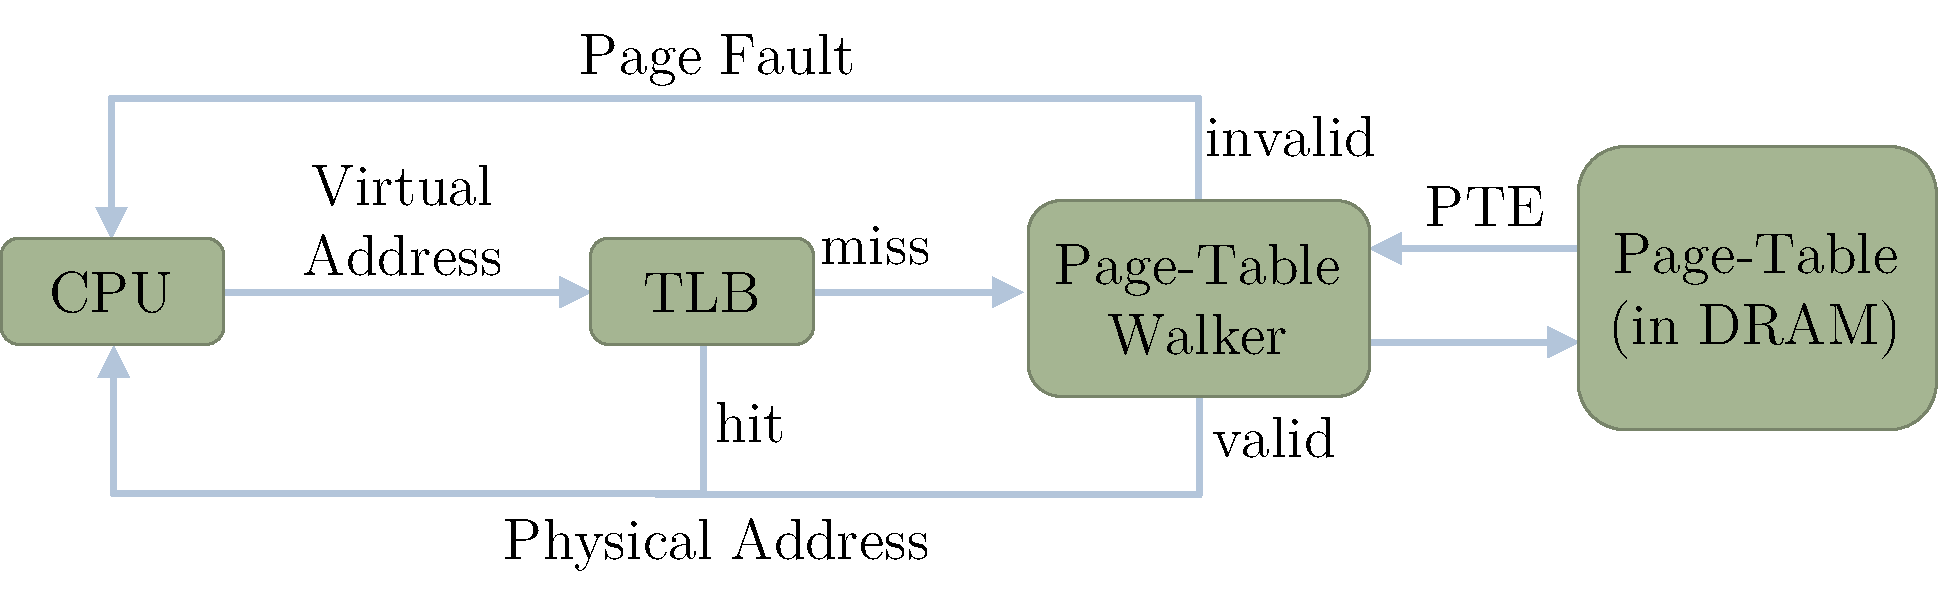
\includegraphics[width=0.9\columnwidth]{figs/generic_paging.pdf}
    \caption{Flow chart for virtual to physical address look up in a typical
      virtual memory system. The translation look aside buffer (TLB) caches
      translations. The page-table walker (PTW) fetches mappings from main
      memory when the TLB misses. Most mappings are valid and can be returned
      directly to the CPU, but invalid mappings result in a trap to the OS.}
    \label{fig:generic_paging_flow}
\end{figure}

There are three main contributors to page fault time: trap time, processing,
and backing store access. Our experiments on an Intel Haswell CPU (running at
\SI{2.6}{\giga\hertz}) show that it takes approximately \SI{800}{\nano\second}
from the time a fault occurs, to when the OS begins executing the page fault
handler. The OS then spends anywhere from \SIrange{4.5}{13}{\micro\second}
processing the fault. With backing store access times measured in milliseconds
(for e.g. a spinning hard disk), this time is insignificant. However, remote
memory systems promise access latencies on the order of several microseconds,
making page-fault processing a significant overhead.

\begin{figure}[h]
    \centering
    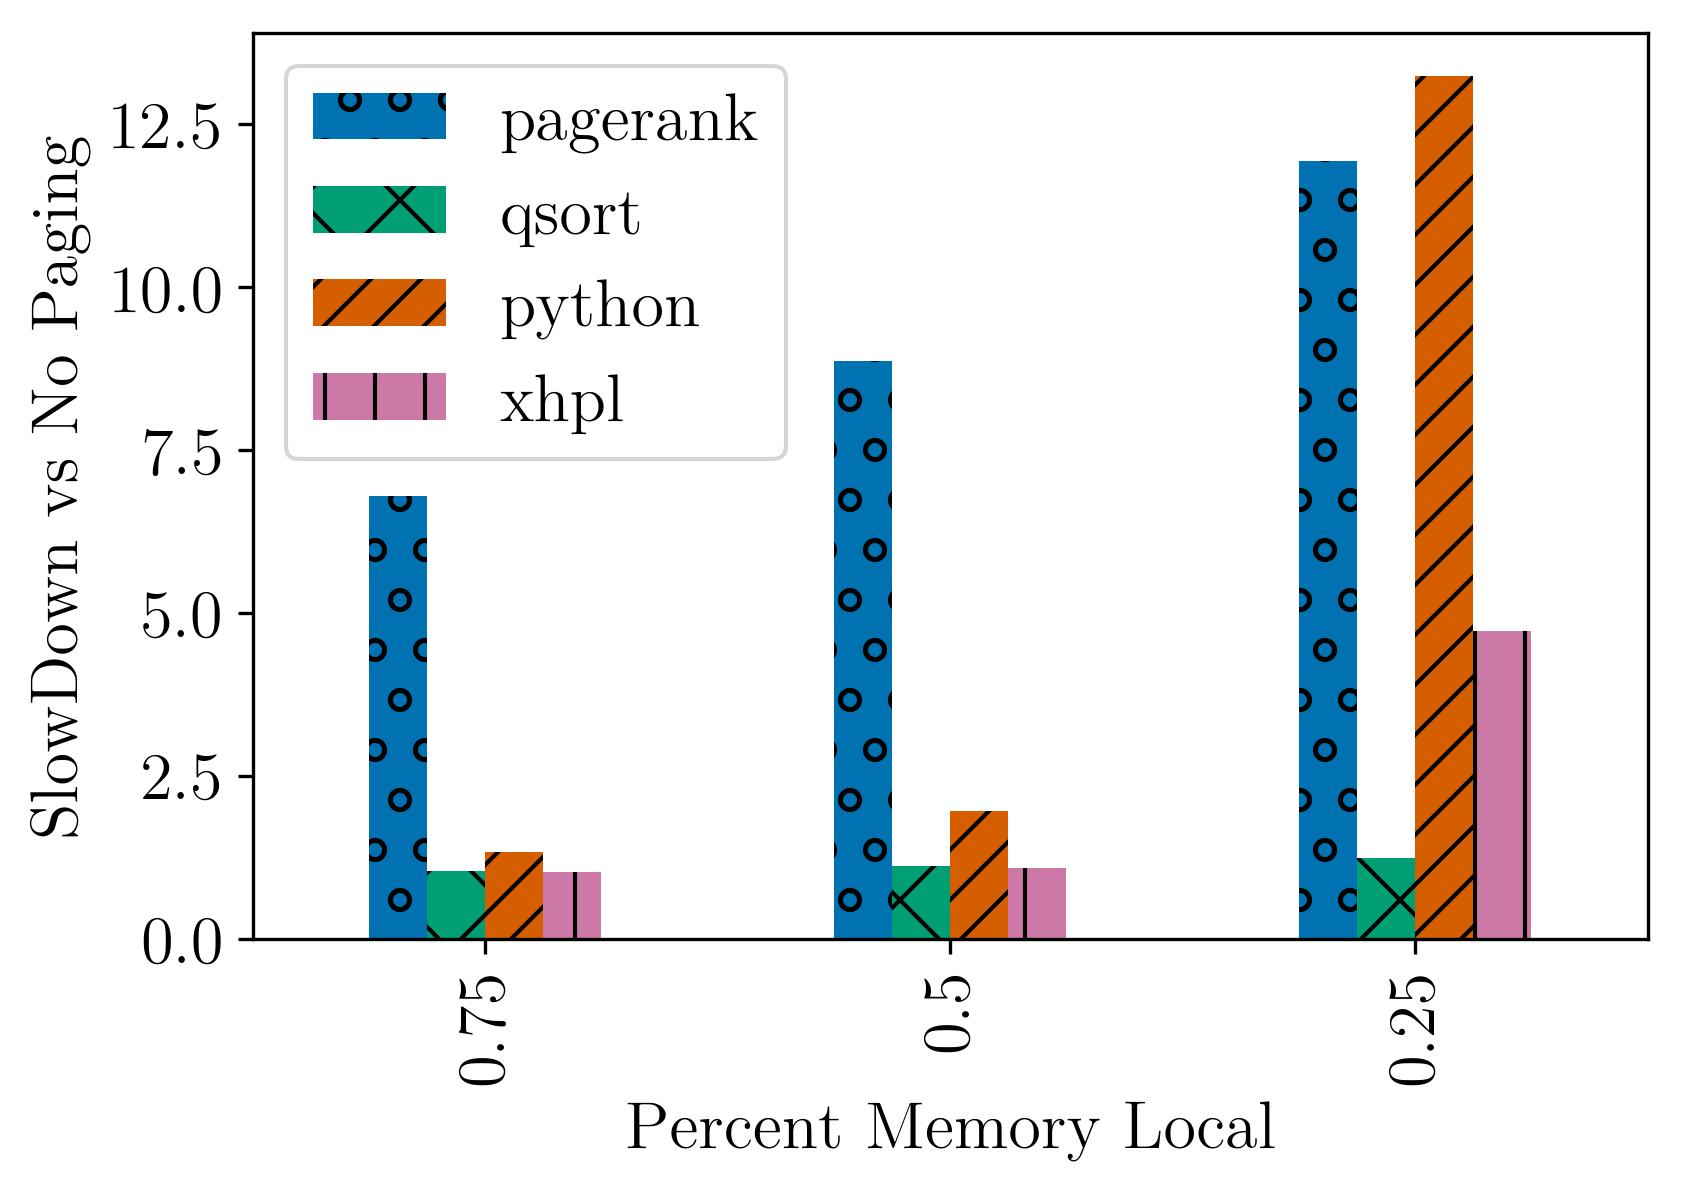
\includegraphics[width=0.9\columnwidth]{figs/paging_overhead.png}
    \caption{Application slow-down when paging to local memory. Memory
oversubscription refers to the percent of peak memory that was stored remotely.}
    \label{fig:paging_overhead}
\end{figure}

To demonstrate this, we modified the Linux kernel to swap to pre-allocated DRAM
buffers in local memory instead of an external device. This effectively
eliminates backing store access times and directly measures the overhead of
using paging at all. Figure \ref{fig:paging_overhead} plots several benchmarks'
runtime as they are run under increasingly memory constrained environments.
Note that even without waiting for secondary storage, applications can slow
down by as much as 12.5x due to paging overheads.

